\section{Phân Tích Các Framework}

  \hspace*{0.8cm}React Native và Flutter là hai framework đa nền tảng phổ biến, mỗi framework mang đến những ưu điểm và thách thức riêng. React Native, phát triển bởi Facebook, cho phép sử dụng JavaScript và tái sử dụng mã nguồn giữa các nền tảng iOS và Android, giúp tiết kiệm chi phí và thời gian phát triển. Với hệ sinh thái phong phú và cộng đồng lớn, React Native dễ dàng tích hợp với các công nghệ khác. Ngược lại, Flutter, do Google phát triển, sử dụng ngôn ngữ Dart và engine render riêng, giúp tối ưu hóa hiệu suất và tạo giao diện người dùng đẹp mắt, đồng thời mang lại hiệu quả cao trong việc phát triển ứng dụng yêu cầu đồ họa phức tạp. Tuy nhiên, Flutter còn thiếu sự phong phú của các plugin và thư viện như React Native. Việc lựa chọn giữa hai framework này phụ thuộc vào yêu cầu dự án, với React Native phù hợp cho các ứng dụng cần phát triển nhanh và dễ dàng tích hợp, còn Flutter thích hợp cho những ứng dụng yêu cầu hiệu suất và giao diện đặc biệt.
\vspace{0.5em}

% 3.1
\subsection{React Native}
\renewcommand{\labelitemi}{--}    
\subsubsection{Kiến Trúc}

\begin{sloppypar}
\hspace*{1.5em}React Native là một framework phát triển ứng dụng đa nền tảng do Meta (trước đây là Facebook) phát triển.  
Nó kết hợp giữa JavaScript và native code để xây dựng ứng dụng di động có giao diện mượt mà và khả năng mở rộng cao.
\end{sloppypar}

\begin{sloppypar}
Kiến trúc của React Native bao gồm ba thành phần chính: \textbf{JavaScript VM}, \textbf{Bridge}, và \textbf{Native Modules}.
\end{sloppypar}

\begin{figure}[H]
    \centering
    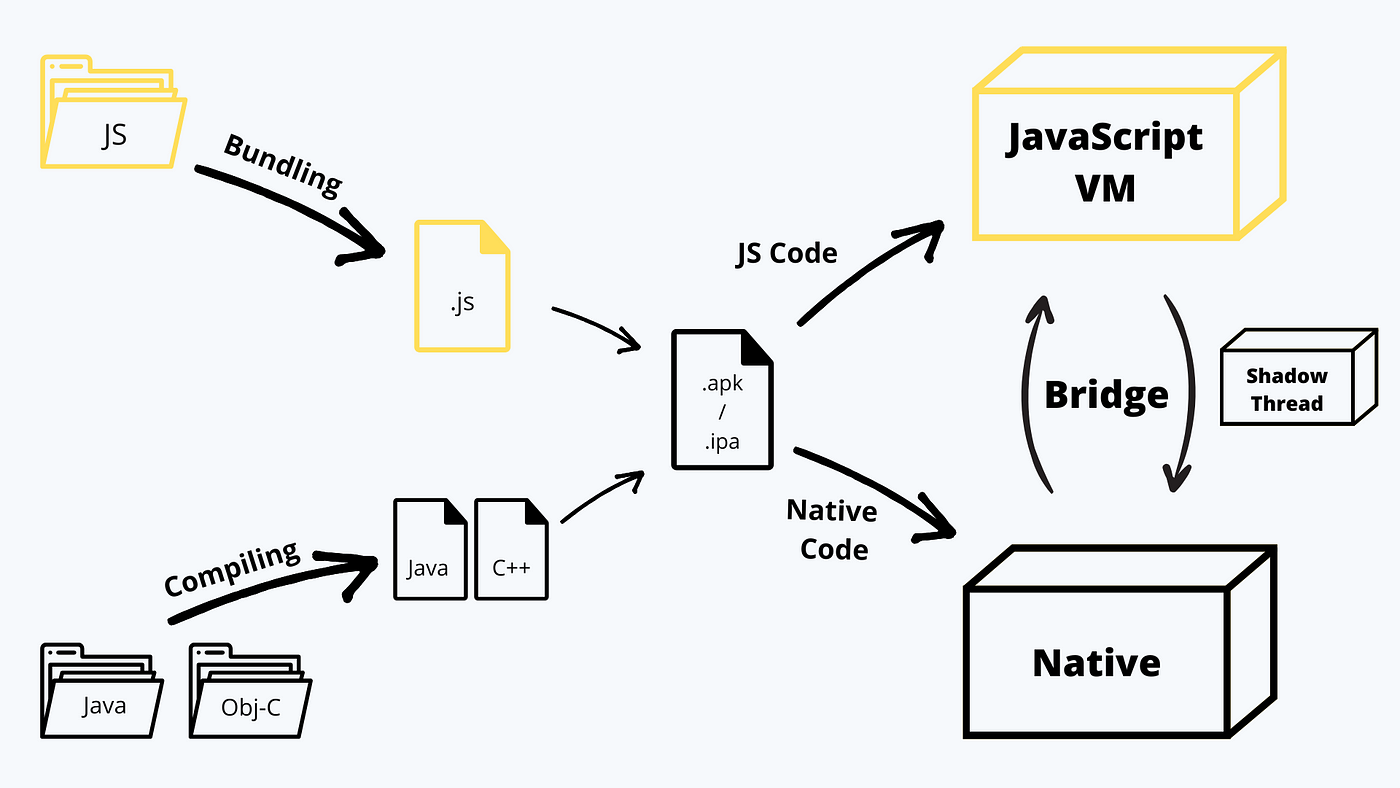
\includegraphics[width=0.95\textwidth]{images/react_native.png}
    \caption{Kiến trúc tổng quan của React Native~\cite{react-native-fabric}}
\end{figure}

\begin{sloppypar}
Trước tiên, JavaScript VM (Virtual Machine) là nơi thực thi logic nghiệp vụ của ứng dụng.  
Khi người dùng tương tác, các hàm JavaScript sẽ xử lý sự kiện, gọi API hoặc thao tác dữ liệu.  
Trên iOS, React Native sử dụng JavaScriptCore của WebKit; trên Android, Meta ưu tiên dùng Hermes – engine nhẹ giúp giảm thời gian khởi động 30\%.  
Ví dụ, Bloomberg đã sử dụng Hermes để tối ưu tốc độ cập nhật dữ liệu chứng khoán thời gian thực.
\end{sloppypar}

\begin{sloppypar}
Tiếp theo, Native Modules là các thành phần được viết bằng ngôn ngữ nền tảng như Java/Kotlin hoặc Obj-C/Swift.  
Chúng cho phép ứng dụng truy cập các API hệ điều hành, ví dụ như GPS hoặc camera.  
Một ví dụ cụ thể là Walmart sử dụng Native Modules để tích hợp thanh toán NFC, đảm bảo hiệu suất và bảo mật cao.
\end{sloppypar}

\begin{sloppypar}
Bridge đóng vai trò là cầu nối giữa JavaScript và native code.  
Khi JavaScript cần gọi chức năng nền tảng, Bridge sẽ truyền dữ liệu qua định dạng JSON – một quy trình tốn thời gian do phải serialize/\-deserialize.  
Theo Đại học Oslo (2022), việc giao tiếp này có thể gây trễ 5–15ms.  
Để khắc phục, Meta giới thiệu kiến trúc mới mang tên Fabric (2023), sử dụng JSI (JavaScript\- Interface) cho phép truy cập trực tiếp native code, giúp cải thiện tốc độ render đến 40\%.
\end{sloppypar}

\subsubsection{Ưu Điểm}
\hspace*{1.5em}React Native mang lại nhiều lợi ích đáng kể, đặc biệt là khả năng tái sử dụng mã nguồn và tốc độ phát triển nhanh.

Một trong những điểm mạnh lớn nhất là khả năng chia sẻ code giữa web và mobile.  
Ví dụ, Airbnb đã tái sử dụng đến 60\% codebase giữa hai nền tảng, tiết kiệm đáng kể thời gian phát triển.  
Thư viện \texttt{React Native Web} giúp chuyển đổi component React Native sang React DOM để chạy trên trình duyệt.

Ngoài ra, hệ sinh thái npm khổng lồ (hơn 2.1 triệu package, 2023) giúp tăng tốc độ lập trình.  
Thư viện như \texttt{React Navigation} đơn giản hóa routing phức tạp, trong khi \texttt{React Native Maps} hỗ trợ hiển thị bản đồ chính xác.

Cuối cùng, React Native cung cấp Live Reload và Hot Reload – hai công cụ giúp lập trình viên cập nhật UI ngay tức thì mà không mất trạng thái.  
Theo khảo sát của JetBrains (2022), tính năng này giúp rút ngắn thời gian debug đến 30\%.

\subsubsection{Nhược Điểm}

\hspace*{1.5em}Dù có nhiều lợi ích, React Native vẫn tồn tại một số hạn chế nhất định, đặc biệt về hiệu năng và khả năng tùy biến.

Do phụ thuộc vào Bridge, hiệu năng ứng dụng thấp hơn so với native.  
Ví dụ, render danh sách 1.000 phần tử trên React Native mất 320ms, trong khi native Android chỉ cần 210ms (Biorn-Hansen, 2021).  
Các ứng dụng yêu cầu đồ họa cao như game 3D hay video editor không phù hợp với React Native.

Một vấn đề khác là phụ thuộc vào thư viện bên thứ ba.  
Khi nền tảng hệ điều hành thay đổi, các thư viện có thể không cập nhật kịp.  
Ví dụ, React Native Firebase gặp lỗi nghiêm trọng khi Android 13 thay đổi cơ chế cấp quyền, gây crash ứng dụng diện rộng.

Cuối cùng, việc tùy chỉnh UI phức tạp như animation nâng cao hay tích hợp OpenGL đòi hỏi viết code native.  
Điều này làm tăng độ phức tạp và yêu cầu đội ngũ có kinh nghiệm phát triển native.

% 3.2
\subsection{Flutter}
\renewcommand{\labelitemi}{--}    
\subsubsection{Kiến Trúc}

\hspace*{1.5em}Flutter là framework đa nền tảng do Google phát triển, sử dụng ngôn ngữ Dart và engine Skia để tự render giao diện người dùng, không phụ thuộc vào thành phần native.

\begin{figure}[H]
    \centering
    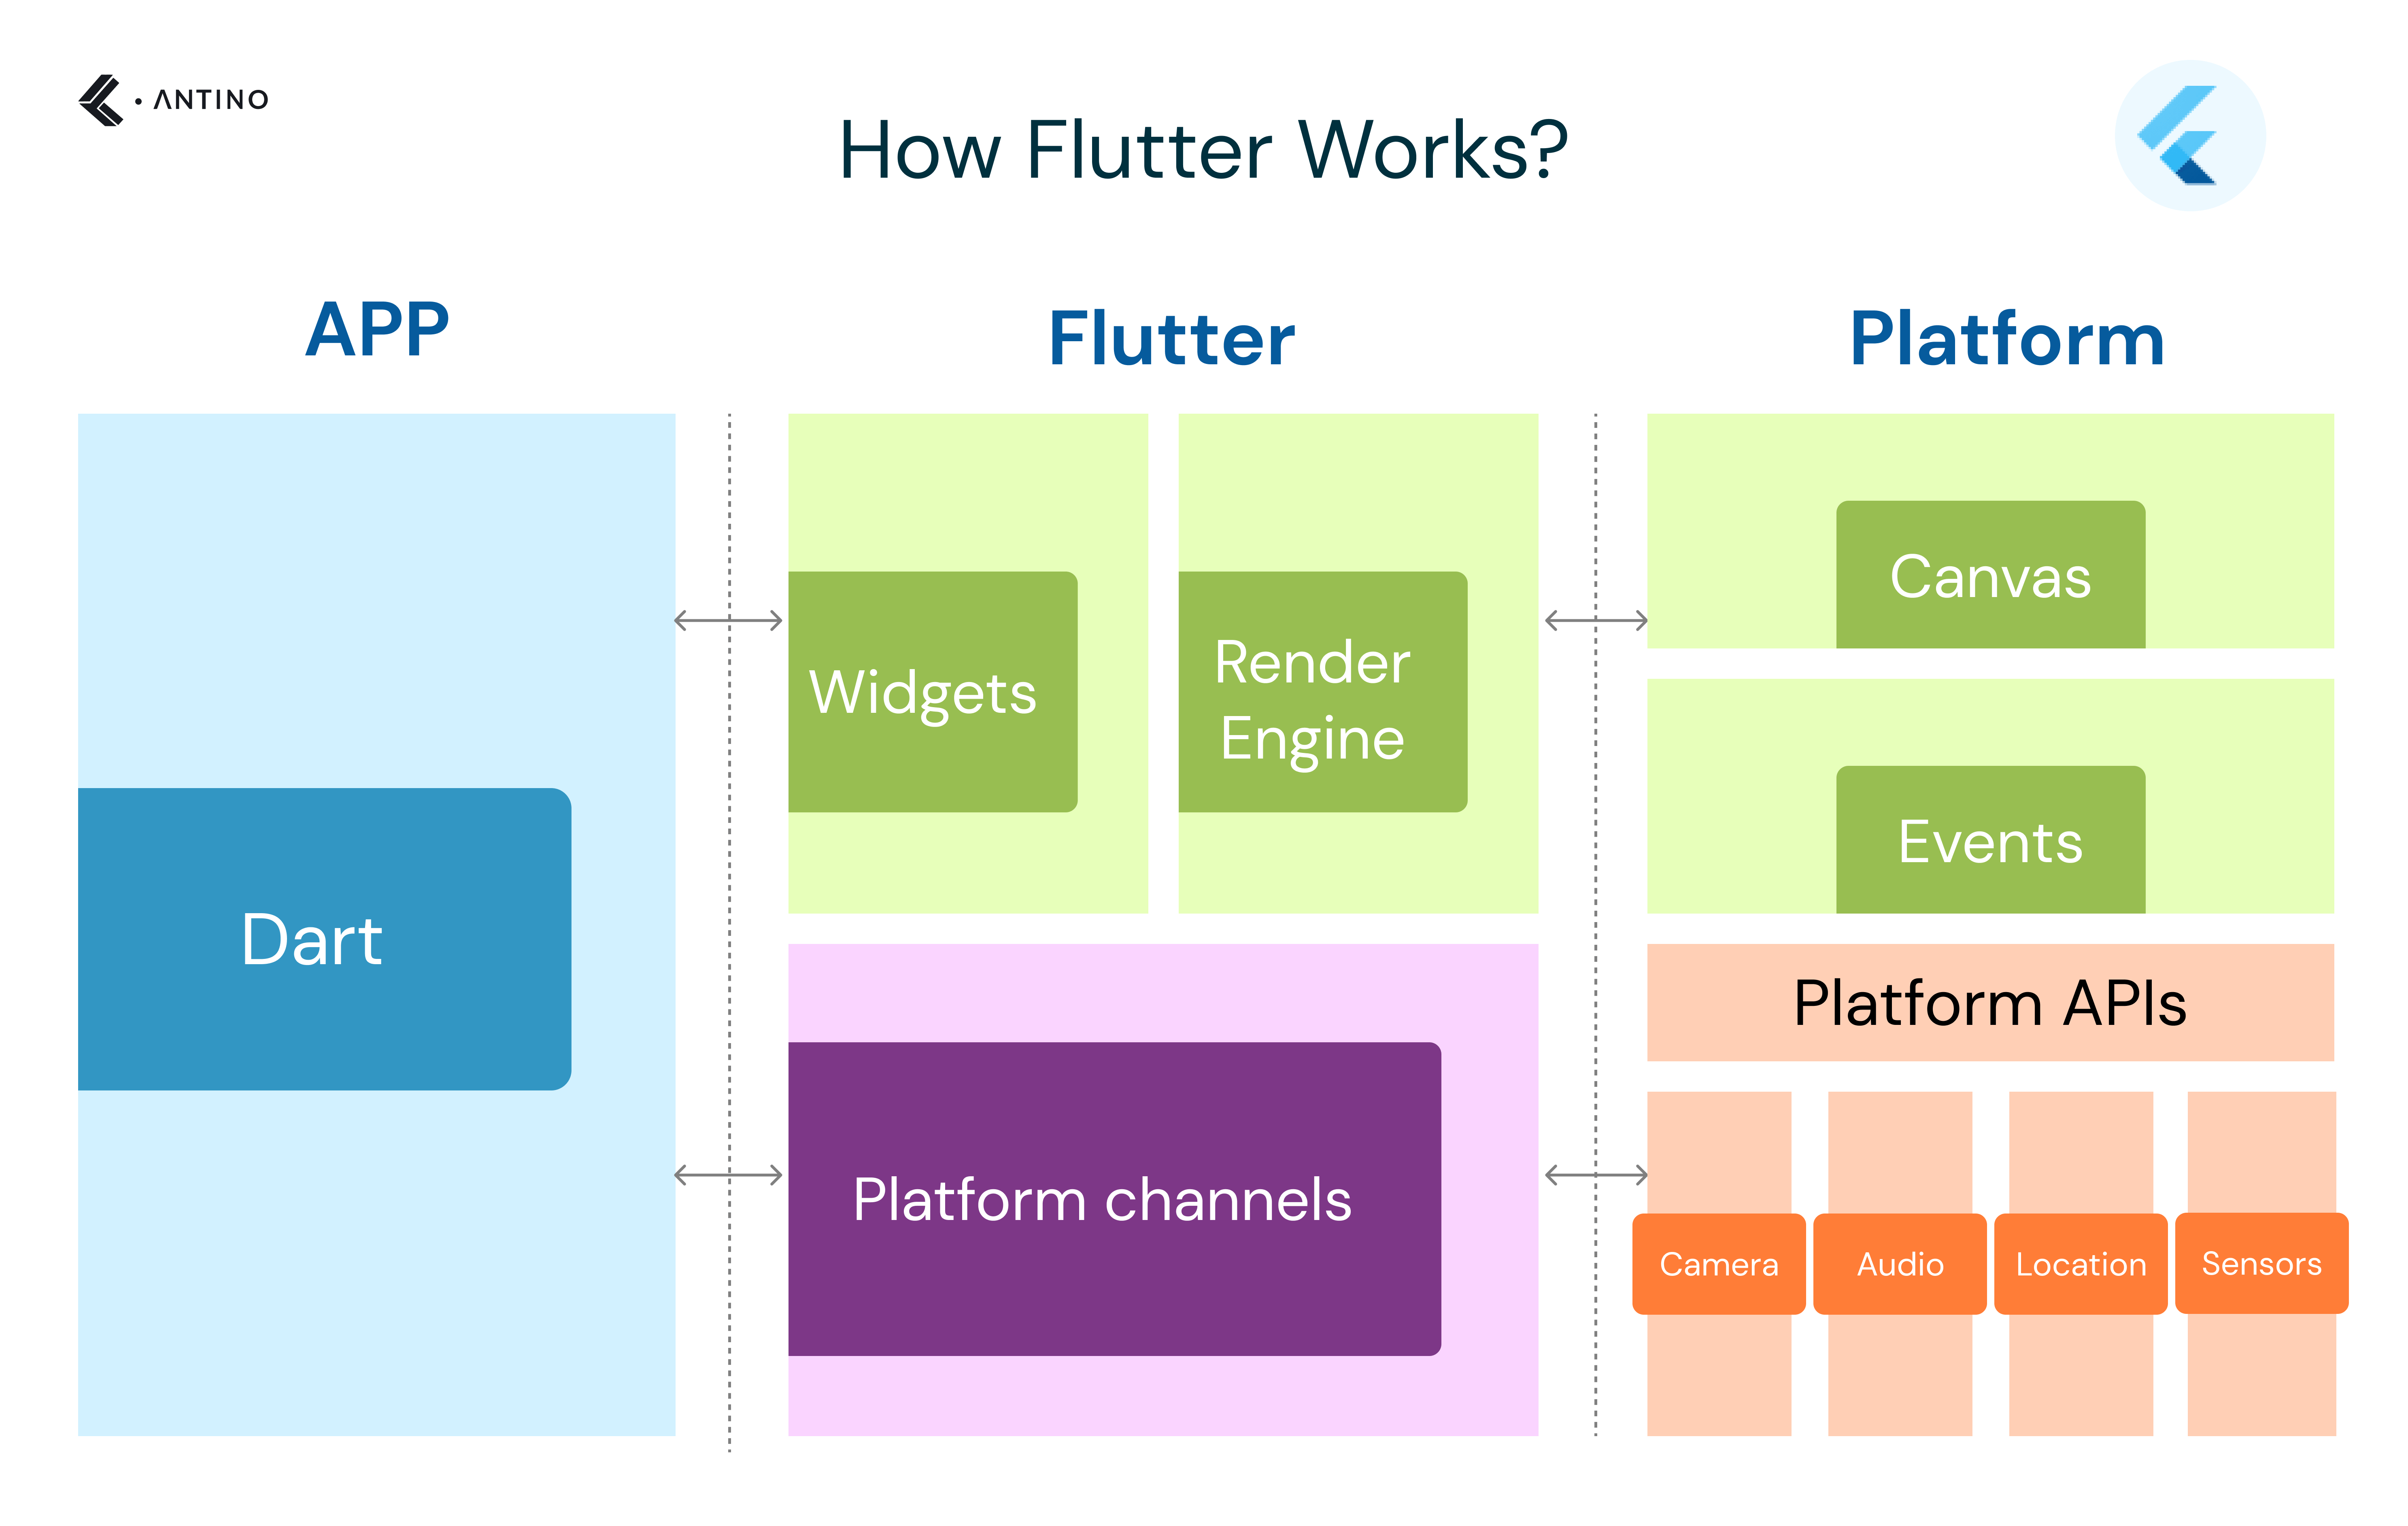
\includegraphics[width=0.9\textwidth]{images/flutter.png}
    \caption{Kiến trúc tổng quan của Flutter} ~\cite{flutter-impeller}
\end{figure}

Dart là ngôn ngữ lập trình cốt lõi của Flutter, được thiết kế để kết hợp hiệu suất cao và tính linh hoạt.  
Dart hỗ trợ hai chế độ biên dịch: AOT (Ahead-of-Time) để tạo mã native tối ưu cho hiệu năng, và JIT (Just-in-Time) cho phép Hot Reload khi phát triển.  
Ví dụ, Alibaba đã dùng Dart để xử lý tới 50 triệu giao dịch/ngày, tận dụng khả năng xử lý bất đồng bộ hiệu quả với \texttt{Future}, \texttt{async/await}.

Tiếp theo, engine Skia là thành phần chịu trách nhiệm vẽ toàn bộ UI lên một canvas duy nhất thay vì sử dụng native widgets.  
Điều này đảm bảo giao diện nhất quán trên mọi nền tảng.  
Chẳng hạn, nút \texttt{ElevatedButton} trong Flutter được render trực tiếp, cho phép tùy biến đến từng pixel.  
Ứng dụng như Starbucks hoặc eBay đã sử dụng Skia để đảm bảo tính thương hiệu trên iOS và Android đồng nhất.

Flutter tổ chức UI theo mô hình widget – mọi thành phần đều là widget, kể cả layout và animation.  
Có hai loại chính:
\begin{itemize}
    \item \textbf{StatelessWidget}: không thay đổi trạng thái (ví dụ: văn bản tĩnh, biểu tượng).
    \item \textbf{StatefulWidget}: có thể thay đổi theo thời gian hoặc tương tác (ví dụ: checkbox, form).
\end{itemize}

Ngoài ra, Flutter hỗ trợ hai thư viện giao diện: \texttt{Material} (Google style) và \texttt{Cupertino} (iOS style), cho phép tạo trải nghiệm quen thuộc tùy theo nền tảng.

Flutter giao tiếp với native thông qua \textbf{Platform Channels}, cho phép gọi các hàm nền tảng như GPS, camera hoặc Bluetooth.  
Ví dụ, khi ứng dụng cần truy cập cảm biến gia tốc, Flutter sẽ gửi message qua channel và native sẽ trả về dữ liệu tương ứng.

\subsubsection{Ưu Điểm}

\hspace*{1.5em}Flutter nổi bật nhờ hiệu năng cao và khả năng tùy chỉnh mạnh:

Thứ nhất, Flutter có hiệu năng gần như native nhờ sử dụng AOT compilation.  
Các ứng dụng như Google Pay đạt 60 FPS ngay cả trên thiết bị cấu hình thấp, với độ trễ phản hồi giao dịch dưới 100ms.

Thứ hai, tính năng \textbf{Hot Reload} cho phép lập trình viên cập nhật giao diện tức thì mà không mất trạng thái ứng dụng.  
Theo báo cáo từ BMW, tính năng này đã giúp nhóm thiết kế UI giảm tới 50\% thời gian phát triển.

Thứ ba, Flutter hỗ trợ đa nền tảng từ một codebase duy nhất, bao gồm Android, iOS, web, Windows, macOS và Linux.  
Ví dụ, ứng dụng Reflectly đạt 95\% tái sử dụng mã nguồn, giúp giảm 70\% chi phí bảo trì so với phát triển riêng lẻ từng nền tảng.

\subsubsection{Nhược Điểm}

\hspace*{1.5em}Mặc dù có nhiều ưu điểm, Flutter vẫn còn một số hạn chế kỹ thuật đáng lưu ý:

Đầu tiên, kích thước ứng dụng Flutter tương đối lớn.  
Một ứng dụng Flutter trống có thể lên đến 20MB, do nhúng sẵn Dart runtime và Skia engine – lớn hơn nhiều so với React Native (khoảng 4MB).  
Điều này ảnh hưởng đến người dùng ở khu vực có tốc độ Internet chậm.

Tiếp theo, lập trình viên phải học ngôn ngữ Dart – vốn chưa phổ biến như JavaScript.  
Cú pháp Dart tương đối mới với nhiều người, đặc biệt trong xử lý bất đồng bộ sử dụng \texttt{Future}, \texttt{Stream} thay vì \texttt{Promise} như trong JS.

Cuối cùng, hệ sinh thái thư viện của Flutter nhỏ hơn React Native.  
Tính đến 2023, Flutter có khoảng 25.000 package trên pub.dev, so với hơn 50.000 package của React Native trên npm.  
Điều này khiến việc tìm thư viện phù hợp đôi khi gặp hạn chế, đặc biệt với các chức năng phức tạp hoặc mới xuất hiện.

% 3.3
\subsection{So sánh React Native và Flutter}
\renewcommand{\labelitemi}{--}

\subsubsection{Hiệu năng khi cuộn (Scrolling)}

  \hspace*{0.8cm}Theo biểu đồ Figure~\ref{fig:scrolling}, Flutter duy trì tốc độ khung hình ổn định gần 60 FPS trong khi React Native có hiện tượng drop mạnh xuống dưới 30 FPS do độ trễ từ bridge giữa UI thread và JavaScript thread. Điều này cho thấy Flutter có hiệu năng cuộn mượt mà hơn, thích hợp với các ứng dụng có nhiều tương tác như game hoặc trình chỉnh sửa ảnh.
\vspace{0.5em}

\begin{figure}[H]
    \centering
    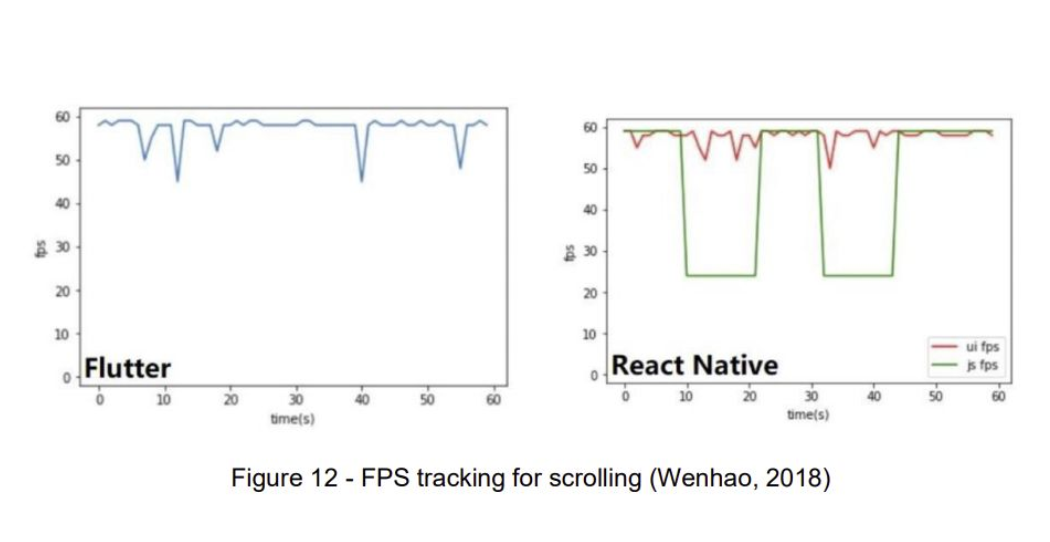
\includegraphics[width=0.8\linewidth]{images/scrolling.png}
    \caption{FPS khi cuộn của Flutter và React Native (Wenhao, 2018)}
    \label{fig:scrolling}
\end{figure}

\subsubsection{Ghi dữ liệu (Write Performance)}

  \hspace*{0.8cm}Biểu đồ Figure~\ref{fig:write} cho thấy thời gian ghi đơn lẻ và trung bình của React Native thấp hơn Flutter, phản ánh hiệu suất tốt hơn ở tác vụ ghi nhẹ. Tuy nhiên, chênh lệch không quá lớn và có thể không đáng kể trong hầu hết ứng dụng thực tế.
\vspace{0.5em}

\begin{figure}[H]
    \centering
    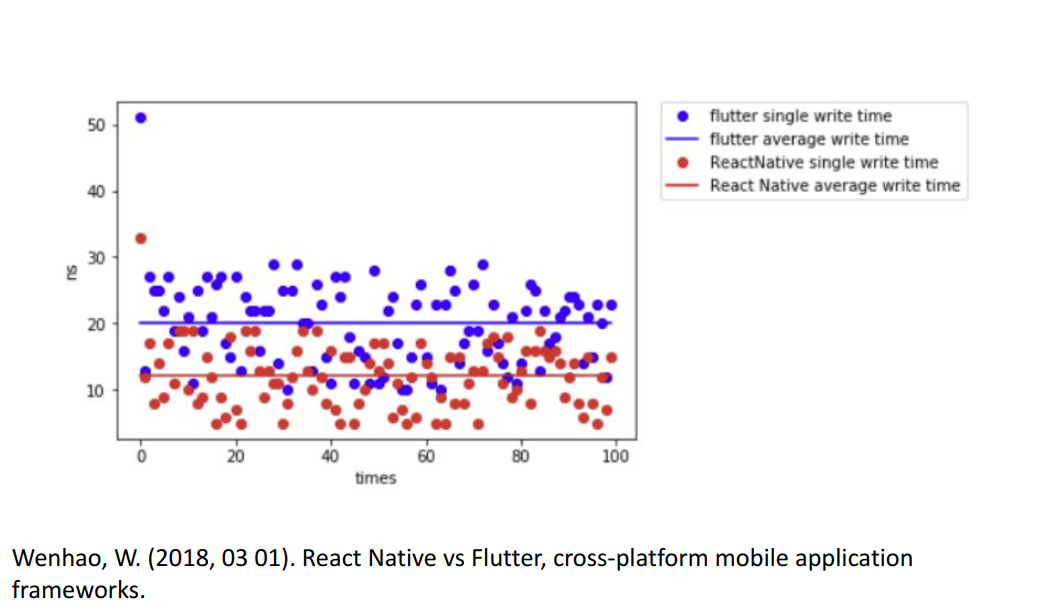
\includegraphics[width=0.8\linewidth]{images/read_write.png}
    \caption{Hiệu suất ghi dữ liệu của Flutter và React Native (Wenhao, 2018)}
    \label{fig:write}
\end{figure}

\subsubsection{Hiệu năng tổng thể theo nghiên cứu mới nhất}

  \hspace*{0.8cm}Theo Biorn-Hansen (2021), React Native và Flutter có điểm tổng thể thấp hơn Native, MAML/MD\textsuperscript{2} và NativeScript về hiệu năng cầu nối (bridge performance). Flutter đạt tổng điểm 15, thấp hơn React Native (16), chủ yếu do sử dụng nhiều RAM tính toán hơn. Tuy nhiên, Flutter vẫn là lựa chọn đáng cân nhắc nếu hiệu năng hình ảnh (UI performance) là yếu tố ưu tiên.
\vspace{0.5em}

\begin{figure}[H]
    \centering
    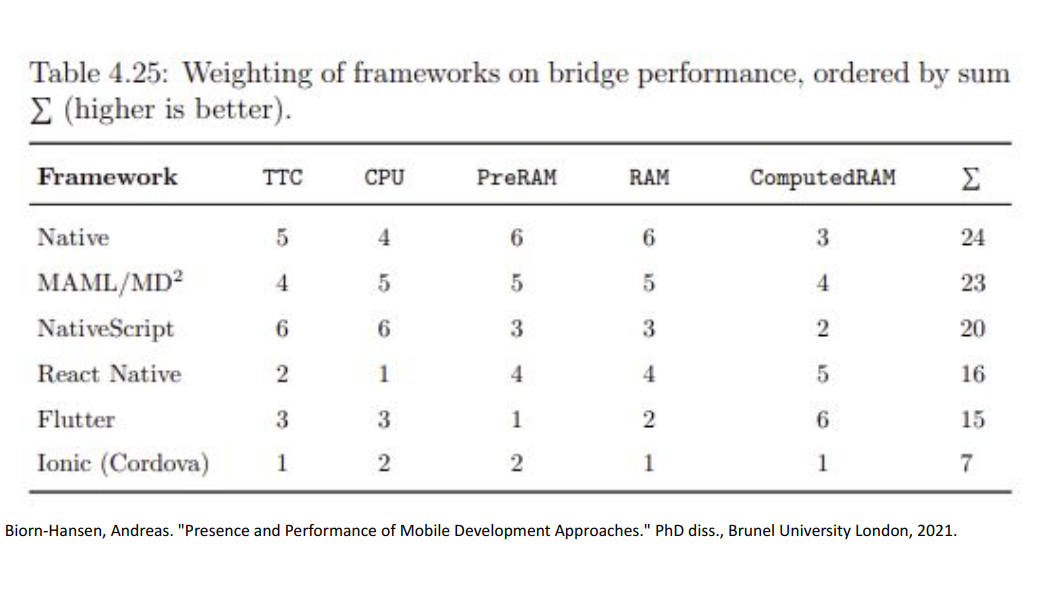
\includegraphics[width=0.7\linewidth]{images/performance.png}
    \caption{Đánh giá hiệu năng framework theo Biorn-Hansen (2021)}
    \label{fig:overall}
\end{figure}

\subsubsection{Ngôn ngữ lập trình}

  \hspace*{0.8cm}React Native sử dụng JavaScript – một ngôn ngữ phổ biến, dễ học, hỗ trợ từ hệ sinh thái Node.js và thư viện lớn. Trong khi đó, Flutter dùng Dart – một ngôn ngữ được Google phát triển với ưu điểm về type safety và khả năng biên dịch AOT, giúp giảm lỗi runtime nhưng đòi hỏi thời gian làm quen.
\vspace{0.5em}

\subsubsection{Phát triển đa nền tảng}

  \hspace*{0.8cm}React Native chủ yếu nhắm đến iOS và Android, tuy có hỗ trợ web nhưng chưa ổn định. Ngược lại, Flutter hỗ trợ 6 nền tảng gồm mobile, web và desktop (Windows, macOS, Linux), phù hợp với ứng dụng cần độ bao phủ rộng và giao diện đồng nhất.
\vspace{0.5em}

\subsubsection{Cộng đồng và tài nguyên}

  \hspace*{0.8cm}React Native sở hữu cộng đồng lớn với hơn 2 triệu developer, tài nguyên phong phú trên Stack Overflow, GitHub và blog kỹ thuật. Flutter tuy mới hơn nhưng đang tăng trưởng nhanh, đặc biệt ở thị trường châu Á, được Google đầu tư mạnh về tài liệu và hỗ trợ chính thức.
\vspace{0.5em}

% 3.4
\subsection{Case Study}
\renewcommand{\labelitemi}{--}    
\subsubsection{React Native: Instagram}

  \hspace*{0.8cm}Instagram đã tích hợp React Native vào ứng dụng native hiện có nhằm tăng tốc độ phát triển các tính năng như \textit{Stories} và giao diện máy ảnh (\textit{Camera UI}). Một trong những thách thức chính là đảm bảo hiệu năng ổn định trên các thiết bị cũ như iPhone 6s. Đội ngũ phát triển đã áp dụng kỹ thuật \textit{lazy loading} để tải component khi cần thiết và tối ưu cầu nối (\textit{bridge}) bằng cách giảm thiểu số lần tương tác giữa JavaScript và native thread. Kết quả, họ tái sử dụng được khoảng 85\% mã nguồn giữa hai nền tảng iOS và Android, đồng thời rút ngắn 30\% thời gian phát triển tính năng.
\vspace{0.5em}

\subsubsection{Flutter: Google Ads}

  \hspace*{0.8cm}Ứng dụng Google Ads được xây dựng bằng Flutter nhằm hỗ trợ quản lý quảng cáo trên nhiều nền tảng. Ứng dụng này xử lý trung bình 5 triệu request mỗi ngày từ 16 quốc gia, với yêu cầu độ trễ phản hồi không vượt quá 200ms. Nhóm phát triển đã tận dụng \textit{Dart isolates} để thực hiện các tác vụ tính toán nặng ở luồng phụ, kết hợp với Firebase để đồng bộ dữ liệu thời gian thực (\textit{real-time}). Kết quả là thời gian tải dữ liệu giảm 40\%, đồng thời giao diện người dùng duy trì tốc độ khung hình 60 FPS trên tất cả thiết bị, bao gồm cả thiết bị cấu hình thấp.
\vspace{0.5em}

% 3.5
\subsection{Kết Luận}
\renewcommand{\labelitemi}{--}    

  \hspace*{0.8cm}Cả React Native và Flutter đều là những framework hàng đầu cho phát triển ứng dụng đa nền tảng. Tuy nhiên, mỗi công nghệ lại phù hợp với những mục tiêu và điều kiện cụ thể trong quá trình phát triển.
  
  \setlength{\leftmargini}{1.5cm}
  \begin{itemize}
    \item Đối với các startup mong muốn đưa sản phẩm ra thị trường nhanh chóng, React Native là lựa chọn lý tưởng nhờ khả năng tái sử dụng mã JavaScript và cộng đồng phát triển rộng lớn.
    \item Trong khi đó, Flutter thể hiện ưu thế vượt trội ở những dự án yêu cầu hiệu năng cao và giao diện người dùng tuỳ chỉnh phức tạp nhờ engine đồ hoạ tích hợp và khả năng biên dịch trực tiếp sang mã máy.
  \end{itemize}
\vspace{0.5em}


  \hspace*{0.8cm}Trong tương lai, cả hai framework đều đang theo đuổi các hướng phát triển mới nhằm mở rộng phạm vi ứng dụng.

  \setlength{\leftmargini}{1.5cm}
  \begin{itemize}
    \item Flutter được kỳ vọng sẽ mở rộng sang các hệ thống nhúng như thiết bị IoT hoặc ô tô thông minh, đặc biệt thông qua dự án Hummingbird.
    \item Ngược lại, React Native đang tập trung vào cải thiện hiệu năng lõi bằng các sáng kiến như Fabric và TurboModules, giúp tối ưu giao tiếp giữa native và JavaScript.
  \end{itemize}
\vspace{0.5em}


  \hspace*{0.8cm}Việc lựa chọn framework phù hợp nên dựa trên các tiêu chí rõ ràng về kỹ thuật và nguồn lực.

  \setlength{\leftmargini}{1.5cm}
  \begin{itemize}
    \item Trước khi quyết định, nhóm phát triển nên đánh giá yêu cầu về giao diện, hiệu năng, cũng như kỹ năng sẵn có trong đội ngũ.
    \item Bên cạnh đó, việc xây dựng nguyên mẫu (\textit{prototype}) bằng cả hai công nghệ để kiểm thử hiệu suất thực tế là cách tiếp cận thực tiễn và hiệu quả.
  \end{itemize}
\vspace{0.5em}
